% answers.tex —— 2007 年·北京卷·理科 · 参考答案与详细解析片段
% 由 tools/generate_projects.py 依来源总账自 2007/2007_数学真题_北京理_试题.md + 2007/2007_数学真题_北京理_解析正文.md + 2007/2007_数学真题_北京理_答案要点.md 生成，勿手改（改源 MD 后重跑）


\begin{gktip}
固定源 PDF 未附答案或解析。以下为编者独立推导并经独立交叉复核，不代表官方答案或官方解析。题面发布者、出版信息、版本和官方身份未核实。
\end{gktip}

\gkpart{一、选择题}

\begin{answer}
\gksolhead{1}{}

\textbf{题目}：

已知 $\cos\theta\cdot\tan\theta<0$，那么角 $\theta$ 是（　）

（A）第一或第二象限角　（B）第二或第三象限角　（C）第三或第四象限角　（D）第一或第四象限角

\Needspace{4\baselineskip}
\textbf{解析}

$\cos\theta\tan\theta=\sin\theta$（原式要求 $\cos\theta\ne0$），故条件等价于 $\sin\theta<0$，即第三或第四象限角，选 \textbf{C}。

\gkanswer{答案：C}

\end{answer}
\begin{answer}
\gksolhead{2}{}

\textbf{题目}：

函数 $f(x)=3^x\ (0<x\leq 2)$ 的反函数的定义域为（　）

（A）$(0,+\infty)$　（B）$(1,9]$　（C）$(0,1)$　（D）$[9,+\infty)$

\Needspace{4\baselineskip}
\textbf{解析}

$f(x)=3^x$ 在 $0<x\le2$ 上的值域是 $(1,9]$，这就是反函数的定义域，选 \textbf{B}。

\gkanswer{答案：B，$(1,9]$}

\end{answer}
\begin{answer}
\gksolhead{3}{}

\textbf{题目}：

平面 $\alpha\parallel$ 平面 $\beta$ 的一个充分条件是（　）

（A）存在一条直线 $a$，$a\parallel\alpha,\ a\parallel\beta$

（B）存在一条直线 $a$，$a\subset\alpha,\ a\parallel\beta$

（C）存在两条平行直线 $a,b$，$a\subset\alpha,\ b\subset\beta,\ a\parallel\beta,\ b\parallel\alpha$

（D）存在两条异面直线 $a,b$，$a\subset\alpha,\ b\subset\beta,\ a\parallel\beta,\ b\parallel\alpha$

\Needspace{4\baselineskip}
\textbf{解析}

若 $\alpha,\beta$ 相交，其交线同时平行于题设的 $a,b$，于是 $a\parallel b$，与 $a,b$ 异面矛盾。因此两平面平行，选 \textbf{D}。

\gkanswer{答案：D}

\end{answer}
\begin{answer}
\gksolhead{4}{}

\textbf{题目}：

已知 $O$ 是 $\triangle ABC$ 所在平面内一点，$D$ 为 $BC$ 边中点，且
$2\overrightarrow{OA}+\overrightarrow{OB}+\overrightarrow{OC}=\vec{0}$，那么（　）

（A）$\overrightarrow{AO}=\overrightarrow{OD}$　（B）$\overrightarrow{AO}=2\overrightarrow{OD}$　（C）$\overrightarrow{AO}=3\overrightarrow{OD}$　（D）$2\overrightarrow{AO}=\overrightarrow{OD}$

\Needspace{4\baselineskip}
\textbf{解析}

记 $\overrightarrow{OA}=\mathbf u$。由 $D$ 为 $BC$ 中点，$\overrightarrow{OD}=\tfrac12(\overrightarrow{OB}+\overrightarrow{OC})=-\mathbf u$，故 $\overrightarrow{AO}=-\mathbf u=\overrightarrow{OD}$，选 \textbf{A}。

\gkanswer{答案：A}

\end{answer}
\begin{answer}
\gksolhead{5}{}

\textbf{题目}：

记者要为 5 名志愿者和他们帮助的 2 位老人拍照，要求排成一排，2 位老人相邻但不排在两端，不同的排法共有（　）

（A）1440 种　（B）960 种　（C）720 种　（D）480 种

\Needspace{4\baselineskip}
\textbf{解析}

将两位老人视为一个相邻整体。该整体不得占两端，故可占第2至第5位中的4个起始位置；老人内部有 $2!$ 种排法，其余5名志愿者有 $5!$ 种排法。总数为 $4\cdot2!\cdot5!=960$，选 \textbf{B}。

\gkanswer{答案：B}

\end{answer}
\begin{answer}
\gksolhead{6}{}

\textbf{题目}：

\Needspace{5\baselineskip}
若不等式组

\nopagebreak[4]
\[
\begin{cases}
x-y\geq 0,\\
2x+y\leq 2,\\
y\geq 0,\\
x+y\leq a,
\end{cases}
\]

表示的平面区域是一个三角形，则 $a$ 的取值范围是（　）

（A）$a\geq\dfrac43$　（B）$0<a\leq 1$　（C）$1\leq a\leq\dfrac43$　（D）$0<a\leq 1$ 或 $a\geq\dfrac43$

\Needspace{4\baselineskip}
\textbf{解析}

不等式组前三个条件围成顶点为 $(0,0),(1,0),(2/3,2/3)$ 的三角形。直线 $x+y=a$ 从原点方向切入：$0<a\le1$ 时截得三角形；$1<a<4/3$ 时截得四边形；$a\ge4/3$ 时不再削去原三角形内部。因此所求为 $0<a\le1$ 或 $a\ge4/3$，选 \textbf{D}。

\gkanswer{答案：D，$0<a\leq1$ 或 $a\geq\dfrac43$}

\end{answer}
\begin{answer}
\gksolhead{7}{}

\textbf{题目}：

如果正数 $a,b,c,d$ 满足 $a+b=cd=4$，那么（　）

（A）$ab\leq c+d$，且等号成立时 $a,b,c,d$ 的取值唯一

（B）$ab\geq c+d$，且等号成立时 $a,b,c,d$ 的取值唯一

（C）$ab\leq c+d$，且等号成立时 $a,b,c,d$ 的取值不唯一

（D）$ab\geq c+d$，且等号成立时 $a,b,c,d$ 的取值不唯一

\Needspace{4\baselineskip}
\textbf{解析}

由 $a+b=4$，$ab\le(a+b)^2/4=4$，等号当且仅当 $a=b=2$。又 $cd=4$ 且 $c,d>0$，故 $c+d\ge2\sqrt{cd}=4$，等号当且仅当 $c=d=2$。于是 $ab\le c+d$；总等号仅在 $a=b=c=d=2$ 成立，取值唯一，选 \textbf{A}。

\gkanswer{答案：A}

\end{answer}
\begin{answer}
\gksolhead{8}{}

\textbf{题目}：

对于函数① $f(x)=\lg(|x-2|+1)$，② $f(x)=(x-2)^2$，③ $f(x)=\cos(x+2)$，判断如下三个命题的真假：

命题甲：$f(x+2)$ 是偶函数；

命题乙：$f(x)$ 在 $(-\infty,2)$ 上是减函数，在 $(2,+\infty)$ 上是增函数；

命题丙：$f(x+2)-f(x)$ 在 $(-\infty,+\infty)$ 上是增函数。

能使命题甲、乙、丙均为真的所有函数的序号是（　）

（A）①③　（B）①②　（C）③　（D）②

\Needspace{4\baselineskip}
\textbf{解析}

对①，$f(x+2)=\lg(|x|+1)$ 为偶函数，且 $f$ 在2两侧分别递减、递增；但当 $x>2$ 时，$f(x+2)-f(x)=\lg\dfrac{x+1}{x-1}$ 随 $x$ 增大而减小，故丙不成立。②平移后为 $x^2$，甲、乙成立；其差 $f(x+2)-f(x)=x^2-(x-2)^2=4x-4$ 为增函数。③有 $f(x+2)=\cos(x+4)$，不是偶函数，且原函数在 $(-\infty,2)$ 上并非单调递减。因此只有②，选 \textbf{D}。

\gkanswer{答案：D（②）}

\end{answer}
\gkpart{二、填空题}

\begin{answer}
\gksolhead{9}{}

\textbf{题目}：

$\dfrac{2}{(1+i)^2}=$\gkblank{}。

\Needspace{4\baselineskip}
\textbf{解析}

$(1+i)^2=2i$，所以 $\dfrac2{(1+i)^2}=1/i=-i$。

\gkanswer{答案：$-i$}

\end{answer}
\begin{answer}
\gksolhead{10}{}

\textbf{题目}：

若数列 $\{a_n\}$ 的前 $n$ 项和 $S_n=n^2-10n\ (n=1,2,3,\ldots)$，则此数列的通项公式为\gkblank{}；数列 $\{na_n\}$ 中数值最小的项是第\gkblank{}项。

\Needspace{4\baselineskip}
\textbf{解析}

$a_1=S_1=-9$。对 $n\ge2$，$a_n=S_n-S_{n-1}=2n-11$；该式对 $n=1$ 也成立。于是 $na_n=2n^2-11n$，在正整数 $n$ 中最小值于 $n=3$ 取得。填 $2n-11$，第3项。

\gkanswer{答案：$a_n=2n-11$；第 3 项}

\end{answer}
\begin{answer}
\gksolhead{11}{}

\textbf{题目}：

在 $\triangle ABC$ 中，若 $\tan A=\dfrac13$，$C=150^\circ$，$BC=1$，则 $AB=$\gkblank{}。

\Needspace{4\baselineskip}
\textbf{解析}

$\tan A=1/3>0$，且 $A$ 是三角形内角，故 $A$ 为锐角、$\sin A=1/\sqrt{10}$。正弦定理给出
$AB=BC\cdot\dfrac{\sin C}{\sin A}=1\cdot\dfrac{1/2}{1/\sqrt{10}}=\dfrac{\sqrt{10}}2$。

\gkanswer{答案：$\dfrac{\sqrt{10}}2$}

\end{answer}
\begin{answer}
\gksolhead{12}{}

\textbf{题目}：

已知集合 $A=\{x\mid |x-a|\leq 1\}$，$B=\{x\mid x^2-5x+4\geq 0\}$。若 $A\cap B=\varnothing$，则实数 $a$ 的取值范围是\gkblank{}。

\Needspace{4\baselineskip}
\textbf{解析}

$B=(-\infty,1]\cup[4,+\infty)$，$A=[a-1,a+1]$。区间 $A$ 与 $B$ 不相交当且仅当 $a-1>1$ 且 $a+1<4$，即 $2<a<3$。

\gkanswer{答案：$(2,3)$}

\end{answer}
\begin{answer}
\gksolhead{13}{}

\textbf{题目}：

2002 年在北京召开的国际数学家大会，会标是以我国古代数学家赵爽的弦图为基础设计的。弦图是由四个全等直角三角形与一个小正方形拼成的一个大正方形（如图）。如果小正方形的面积为 1，大正方形的面积为 25，直角三角形中较小的锐角为 $\theta$，那么 $\cos 2\theta$ 的值等于\gkblank{}。
\nopagebreak[4]
\begin{center}% 依据固定来源 PDF 第 1 页重绘；source_id=src-3612a22ce3848ad6ebbec4d94861dd64b009980e14e8c7a83efefb2ea39bd367
% PDF SHA-256: 2cea664b02860c04aa21fb6bdf80403b674befb8e61fa9f68970197bdf0f5ff4
\begin{center}
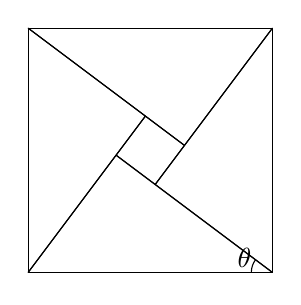
\begin{tikzpicture}[scale=0.62,line join=round,line cap=round]
  \coordinate (A) at (0,0);
  \coordinate (B) at (5,0);
  \coordinate (C) at (5,5);
  \coordinate (D) at (0,5);
  \coordinate (P) at (1.8,2.4);
  \coordinate (Q) at (2.6,1.8);
  \coordinate (R) at (3.2,2.6);
  \coordinate (S) at (2.4,3.2);
  \draw (A)--(B)--(C)--(D)--cycle;
  \draw (A)--(P)--(B);
  \draw (B)--(Q)--(C);
  \draw (C)--(R)--(D);
  \draw (D)--(S)--(A);
  \draw (P)--(Q)--(R)--(S)--cycle;
  \draw (4.57,0) arc[start angle=180,end angle=143.13,radius=0.43];
  \node at (4.43,0.30) {$\theta$};
\end{tikzpicture}
\end{center}
\end{center}
\nopagebreak[4]
\Needspace{4\baselineskip}
\textbf{解析}

设直角三角形长、短直角边分别为 $L,S$。中央正方形边长为 $L-S=1$，大正方形边长是斜边，故 $L^2+S^2=25$。由 $(L-S)^2=L^2+S^2-2LS=1$ 得 $LS=12$，从而 $L+S=7$。较小锐角对着短直角边，故
$\cos2\theta=(L^2-S^2)/(L^2+S^2)=(L-S)(L+S)/25=7/25$。

\gkanswer{答案：$\dfrac7{25}$}

\end{answer}
\begin{answer}
\gksolhead{14}{}

\textbf{题目}：

已知函数 $f(x)$，$g(x)$ 分别由下表给出：

\begin{center}
\begin{tabular}{lrrr}
\toprule
$x$ & 1 & 2 & 3 \\
\midrule
$f(x)$ & 1 & 3 & 1 \\
\bottomrule
\end{tabular}
\end{center}

\begin{center}
\begin{tabular}{lrrr}
\toprule
$x$ & 1 & 2 & 3 \\
\midrule
$g(x)$ & 3 & 2 & 1 \\
\bottomrule
\end{tabular}
\end{center}

则 $f[g(1)]$ 的值为\gkblank{}；满足 $f[g(x)]>g[f(x)]$ 的 $x$ 的值是\gkblank{}。

\Needspace{4\baselineskip}
\textbf{解析}

$g(1)=3$，所以 $f[g(1)]=f(3)=1$。分别代入 $x=1,2,3$ 检查复合函数不等式，只有 $x=2$ 成立。

\gkanswer{答案：$1$；$x=2$}

\end{answer}
\gkpart{三、解答题}

\begin{answer}
\gksolhead{15}{}

\textbf{题目}：

数列 $\{a_n\}$ 中，$a_1=2,\ a_{n+1}=a_n+cn$（$c$ 是常数，$n=1,2,3,\ldots$），且 $a_1,a_2,a_3$ 成公比不为 1 的等比数列。

（1） 求 $c$ 的值；

（2） 求 $\{a_n\}$ 的通项公式。

\Needspace{4\baselineskip}
\textbf{解析}

\textbf{（1）} $a_2=2+c$，$a_3=2+3c$。三项成等比数列给出 $(2+c)^2=2(2+3c)$，即 $c(c-2)=0$。$c=0$ 会使公比为1，故 $c=2$。

\textbf{（2）} 递推求和：$a_n=2+2\sum_{j=1}^{n-1}j=n^2-n+2$。

\gkanswer{答案（1）：$c=2$}

\gkanswer{答案（2）：$a_n=n^2-n+2$}

\end{answer}
\begin{answer}
\gksolhead{16}{}

\textbf{题目}：

如图，在 $\mathrm{Rt}\triangle AOB$ 中，$\angle OAB=\dfrac{\pi}{6}$，斜边 $AB=4$。$\mathrm{Rt}\triangle AOC$ 可以通过 $\mathrm{Rt}\triangle AOB$ 以直线 $AO$ 为轴旋转得到，且二面角 $B-AO-C$ 是直二面角。动点 $D$ 在斜边 $AB$ 上。

（1） 求证：平面 $COD\perp$ 平面 $AOB$；

（2） 当 $D$ 为 $AB$ 的中点时，求异面直线 $AO$ 与 $CD$ 所成角的大小；

（3） 求 $CD$ 与平面 $AOB$ 所成角的最大值。
\nopagebreak[4]
\begin{center}% 依据固定来源 PDF 第 1 页的点位、棱线和虚实关系重绘；示意图不按比例
% source_id=src-3612a22ce3848ad6ebbec4d94861dd64b009980e14e8c7a83efefb2ea39bd367
% PDF SHA-256: 2cea664b02860c04aa21fb6bdf80403b674befb8e61fa9f68970197bdf0f5ff4
\begin{center}
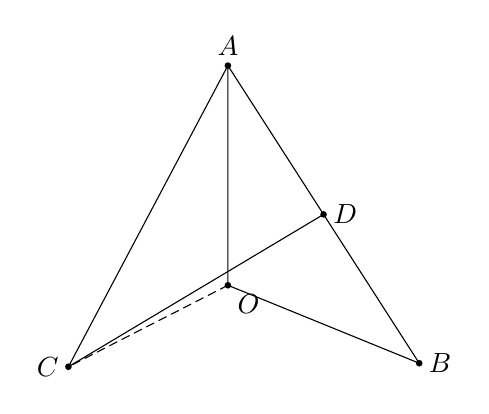
\begin{tikzpicture}[x=0.9cm,y=0.9cm,line join=round,line cap=round]
  \coordinate (A) at (0,3.1);
  \coordinate (O) at (0,0);
  \coordinate (B) at (2.7,-1.1);
  \coordinate (C) at (-2.25,-1.15);
  \coordinate (D) at (1.35,1.0);
  \draw (A)--(B)--(O)--cycle;
  \draw (A)--(C);
  \draw[densely dashed] (O)--(C);
  \draw (C)--(D);
  \fill (A) circle (1.2pt) node[above] {$A$};
  \fill (B) circle (1.2pt) node[right] {$B$};
  \fill (C) circle (1.2pt) node[left] {$C$};
  \fill (O) circle (1.2pt) node[below right] {$O$};
  \fill (D) circle (1.2pt) node[right] {$D$};
\end{tikzpicture}
\end{center}
\end{center}
\nopagebreak[4]
\Needspace{4\baselineskip}
\textbf{解析}

\textbf{（1）} 取坐标 $O=(0,0,0)$，令 $AO$ 为 $x$ 轴。因 $AB=4$ 且 $\angle OAB=\pi/6$，可取 $A=(2\sqrt3,0,0)$、$B=(0,2,0)$；由旋转关系及直二面角可取 $C=(0,0,2)$。点 $D$ 在 $AB$ 上，故 $D$ 在平面 $AOB$ 内；而 $OC\perp$ 平面 $AOB$ 且 $OC\subset$ 平面 $COD$，所以平面 $COD\perp$ 平面 $AOB$。

\textbf{（2）} 当 $D$ 是中点时 $D=(\sqrt3,1,0)$，方向向量 $\overrightarrow{CD}=(\sqrt3,1,-2)$（直线角取锐角），与 $AO$ 方向的夹角满足
$\cos\phi=\sqrt3/\sqrt8=\sqrt6/4$，即 $\phi=\arccos(\sqrt6/4)$。

\textbf{（3）} 令 $D=(2\sqrt3(1-t),2t,0)$，$0\le t\le1$。直线 $CD$ 与平面 $AOB$ 的夹角 $\psi$ 满足
$\sin\psi=2/\sqrt{12(1-t)^2+4t^2+4}=2/\sqrt{16t^2-24t+16}$。
分母平方在 $t=3/4$ 处最小，值为7，故最大夹角为 $\arcsin(2/\sqrt7)$。

\gkanswer{答案（1）：见解析版}

\gkanswer{答案（2）：$\arccos\dfrac{\sqrt6}4$}

\gkanswer{答案（3）：$\arcsin\dfrac2{\sqrt7}$}

\end{answer}
\begin{answer}
\gksolhead{17}{}

\textbf{题目}：

矩形 $ABCD$ 的两条对角线相交于点 $M(2,0)$，$AB$ 边所在直线的方程为 $x-3y-6=0$，点 $T(-1,1)$ 在 $AD$ 边所在直线上。

（1） 求 $AD$ 边所在直线的方程；

（2） 求矩形 $ABCD$ 外接圆的方程；

（3） 若动圆 $P$ 过点 $N(-2,0)$，且与矩形 $ABCD$ 的外接圆外切，求动圆 $P$ 的圆心的轨迹方程。

\Needspace{4\baselineskip}
\textbf{解析}

\textbf{（1）} $AB$ 斜率为 $1/3$，所以 $AD$ 斜率为 $-3$。过 $T(-1,1)$ 得 $AD:3x+y+2=0$；与 $AB:x-3y-6=0$ 相交于 $A=(0,-2)$。

\textbf{（2）} 矩形对角线交点 $M=(2,0)$ 是外接圆圆心，$MA^2=8$，所以圆为 $(x-2)^2+y^2=8$。

\textbf{（3）} 设动圆圆心为 $P$、半径为 $PN$。与圆 $M$ 外切给出 $PM=PN+2\sqrt2$，即 $PM-PN=2\sqrt2$。以 $M,N$ 为焦点，$2a=2\sqrt2$、$c=2$，故 $a^2=b^2=2$，轨迹为 $x^2/2-y^2/2=1$。因 $PM>PN$，取靠近 $N$ 的左支 $x\le-\sqrt2$。

\gkanswer{答案（1）：$3x+y+2=0$}

\gkanswer{答案（2）：$(x-2)^2+y^2=8$}

\gkanswer{答案（3）：$\dfrac{x^2}{2}-\dfrac{y^2}{2}=1$ 的左支}

\end{answer}
\begin{answer}
\gksolhead{18}{}

\textbf{题目}：

某中学号召学生在今年春节期间至少参加一次社会公益活动（以下简称活动），该校合唱团共有 100 名学生，他们参加活动的次数统计如图所示。

图示数据：参加 1 次活动的有 10 人，参加 2 次的有 50 人，参加 3 次的有 40 人；纵轴标“参加人数”，横轴标“活动次数”。

（1） 求合唱团学生参加活动的人均次数；

（2） 从合唱团中任意选两名学生，求他们参加活动次数恰好相等的概率；

（3） 从合唱团中任意选两名学生，用 $\xi$ 表示这两人参加活动次数之差的绝对值，求随机变量 $\xi$ 的分布列及数学期望 $E\xi$。
\nopagebreak[4]
\begin{center}% 依据固定来源 PDF 第 2 页的柱高与坐标轴文字重绘
% source_id=src-3612a22ce3848ad6ebbec4d94861dd64b009980e14e8c7a83efefb2ea39bd367
% PDF SHA-256: 2cea664b02860c04aa21fb6bdf80403b674befb8e61fa9f68970197bdf0f5ff4
\begin{center}
\begin{tikzpicture}[x=0.72cm,y=0.075cm,line join=round]
  \draw[->] (0,0)--(4.7,0) node[right] {活动次数};
  \draw[->] (0,0)--(0,60) node[above] {参加人数};
  \draw (0.65,0) rectangle (1.35,10);
  \draw (1.65,0) rectangle (2.35,50);
  \draw (2.65,0) rectangle (3.35,40);
  \foreach \x/\label in {1/1,2/2,3/3} {
    \draw (\x,0)--(\x,-2.3) node[below] {\label};
  }
  \foreach \y/\label in {10/10,20/20,30/30,40/40,50/50} {
    \draw (-0.08,\y)--(0.08,\y);
    \node[left] at (-0.12,\y) {\label};
  }
\end{tikzpicture}
\end{center}
\end{center}
\nopagebreak[4]
\Needspace{4\baselineskip}
\textbf{解析}

\textbf{（1）} 人均次数为 $(10\cdot1+50\cdot2+40\cdot3)/100=23/10$。

\textbf{（2）} 总选法为 $\binom{100}{2}$，次数相同的选法为 $\binom{10}{2}+\binom{50}{2}+\binom{40}{2}=2050$，概率为 $2050/4950=41/99$。

\textbf{（3）} 两人次数差 $\xi$ 的取值为0、1、2。相应无序选法数分别为2050，$10\cdot50+50\cdot40=2500$，$10\cdot40=400$，故概率分别为 $41/99,50/99,8/99$。于是 $E\xi=(2500+2\cdot400)/4950=2/3$。

\gkanswer{答案（1）：$\dfrac{23}{10}$ 次}

\gkanswer{答案（2）：$\dfrac{41}{99}$}

\gkanswer{答案（3）：$P(\xi=0)=\dfrac{41}{99},\ P(\xi=1)=\dfrac{50}{99},\ P(\xi=2)=\dfrac8{99}$；$E\xi=\dfrac23$}

\end{answer}
\begin{answer}
\gksolhead{19}{}

\textbf{题目}：

如图，有一块半椭圆形钢板，其半轴长为 $2r$，短半轴长为 $r$，计划将此钢板切割成等腰梯形的形状，下底 $AB$ 是半椭圆的短轴，上底 $CD$ 的端点在椭圆上，记 $CD=2x$，梯形面积为 $S$。

（1） 求面积 $S$ 以 $x$ 为自变量的函数式，并写出其定义域；

（2） 求面积 $S$ 的最大值。
\nopagebreak[4]
\begin{center}% 依据固定来源 PDF 第 2 页半椭圆、梯形及两处 2r 尺寸标注重绘
% source_id=src-3612a22ce3848ad6ebbec4d94861dd64b009980e14e8c7a83efefb2ea39bd367
% PDF SHA-256: 2cea664b02860c04aa21fb6bdf80403b674befb8e61fa9f68970197bdf0f5ff4
\begin{center}
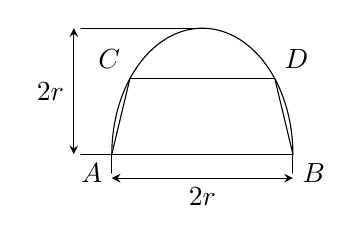
\begin{tikzpicture}[x=1.15cm,y=0.8cm,line join=round,line cap=round,>=stealth]
  \coordinate (A) at (-1,0);
  \coordinate (B) at (1,0);
  \coordinate (C) at (-0.8,1.2);
  \coordinate (D) at (0.8,1.2);
  \draw[domain=180:0,samples=100,smooth,variable=\t] plot ({cos(\t)},{2*sin(\t)});
  \draw (A)--(B);
  \draw (C)--(D);
  \draw (A)--(C);
  \draw (B)--(D);
  \draw[<->] (-1,-0.38)--(1,-0.38) node[midway,below] {$2r$};
  \draw (-1,0)--(-1,-0.30);
  \draw (1,0)--(1,-0.30);
  \draw[<->] (-1.42,0)--(-1.42,2) node[midway,left] {$2r$};
  \draw (-1,0)--(-1.34,0);
  \draw (0,2)--(-1.34,2);
  \node[below left] at (A) {$A$};
  \node[below right] at (B) {$B$};
  \node[above left] at (C) {$C$};
  \node[above right] at (D) {$D$};
\end{tikzpicture}
\end{center}
\end{center}
\nopagebreak[4]
\begin{gktip}

\textbf{原文疑点（ISSUE-1203，未决）}：题干印作“其半轴长为 $2r$，短半轴长为 $r$”；保留原文，未擅自补成“长半轴长”。
\end{gktip}

\Needspace{4\baselineskip}
\textbf{解析}

\textbf{（1）} 按图示尺寸，半椭圆的水平短半轴为 $r$、竖直半轴为 $2r$（图中 $AB=2r$ 且高标 $2r$）。若上底端点横坐标为 $\pm x$，则 $CD=2x$，其高度为 $2r\sqrt{1-x^2/r^2}$。梯形面积
$S=\tfrac12(2r+2x)\,2r\sqrt{1-x^2/r^2}=2(r+x)\sqrt{r^2-x^2}$，非退化情形 $0<x<r$。求导或令 $u=x/r$，可得最大值在 $x=r/2$ 处取得，$S_{\max}=3\sqrt3 r^2/2$。

\textbf{源文疑点（ISSUE-1203，未决并阻断整卷完成）：}题干印作“其半轴长为 $2r$，短半轴长为 $r$”，第一处未明确说明“长半轴”。本推导采用原图尺寸关系；发布前仍需保留该转录疑点，不能把补足后的术语伪装成原文字样。

\textbf{（2）} 面积最大值为 $S_{\max}=3\sqrt3 r^2/2$，在 $x=r/2$ 时取得。

\gkanswer{答案（1）：$S=2(r+x)\sqrt{r^2-x^2}$，$0<x<r$}

\gkanswer{答案（2）：$S_{\max}=\dfrac{3\sqrt3}{2}r^2$}

\end{answer}
\begin{answer}
\gksolhead{20}{}

\textbf{题目}：

\Needspace{5\baselineskip}
已知集合 $A=\{a_1,a_2,\ldots,a_k\}\ (k\geq 2)$，其中 $a_i\in\mathbb{Z}\ (i=1,2,\ldots,k)$。由 $A$ 中的元素构成两个相应的集合：

\nopagebreak[4]
\[
S=\{(a,b)\mid a\in A,\ b\in A,\ a+b\in A\};\qquad
T=\{(a,b)\mid a\in A,\ b\in A,\ a-b\in A\},
\]

其中 $(a,b)$ 是有序数对，集合 $S$ 和 $T$ 中的元素个数分别为 $m$ 和 $n$。若对于任意的 $a\in A$，总有 $-a\notin A$，则称集合 $A$ 具有性质 $P$。

（1） 检验集合 $\{0,1,2,3\}$ 与 $\{-1,2,3\}$ 是否具有性质 $P$，并对其中具有性质 $P$ 的集合，写出相应的集合 $S$ 和 $T$；

（2） 对任何具有性质 $P$ 的集合 $A$，证明：$n\leq \dfrac{k(k-1)}2$；

（3） 判断 $m$ 和 $n$ 的大小关系，并证明你的结论。

\begin{gktip}
\textbf{来源说明}：本题面逐题依据固定来源 PDF（2 页 A3，印刷页码 351–352）转录，source ID 为 \texttt{src-3612a22ce3848ad6ebbec4d94861dd64b009980e14e8c7a83efefb2ea39bd367}，SHA-256 为 \texttt{2cea664b02860c04aa21fb6bdf80403b674befb8e61fa9f68970197bdf0f5ff4}。固定源没有答案、解析或评分标准；发布者、出版信息、版本及官方身份未核。图形尚待矢量重绘。题19“半轴长”按原文保留，术语含义待核。
\end{gktip}

\Needspace{4\baselineskip}
\textbf{解析}

\textbf{（1）} 对 $A=\{0,1,2,3\}$，因 $0=-0\in A$，不具性质 $P$。对 $A=\{-1,2,3\}$，任意元素的相反数均不在 $A$，故具性质 $P$。逐对检验得
$S=\{(-1,3),(3,-1)\}$，$T=\{(2,-1),(2,3)\}$。

\textbf{（2）} 一般地，若 $(a,b)\in T$ 且 $a=b$，则 $0=a-b\in A$，与性质 $P$ 矛盾，故 $T$ 不含对角数对。若 $a\ne b$ 且 $(a,b),(b,a)$ 均在 $T$，则 $a-b,b-a\in A$，两者互为相反数，亦与性质 $P$ 矛盾。因此每个二元无序子集至多对应一个 $T$ 中的有序数对，$n\le\binom{k}{2}$。

\textbf{（3）} 映射 $\varphi:S\to T$ 定义为 $\varphi(a,b)=(a+b,b)$。若 $(a,b)\in S$，则 $a+b,b\in A$ 且 $(a+b)-b=a\in A$，所以 $\varphi(a,b)\in T$。反过来 $(c,b)\in T$ 映到 $(c-b,b)\in S$；两映射互逆，故 $m=n$。

\gkanswer{答案（1）：$\{0,1,2,3\}$ 不具有性质 $P$；$\{-1,2,3\}$ 具有性质 $P$，$S=\{(-1,3),(3,-1)\}$，$T=\{(2,-1),(2,3)\}$}

\gkanswer{答案（2）：$n\leq\dfrac{k(k-1)}2$}

\gkanswer{答案（3）：$m=n$}

\end{answer}